\documentclass[a4paper, 12pt]{report}
\usepackage[utf8x]{inputenc}
\usepackage[francais]{babel}
\usepackage{graphicx}
\usepackage{hyperref}
\title{Génie logiciel et gestion de projet : \\ HomePlans}
\author{Groupe 05}
\begin{document}
\maketitle
	\chapter{Introduction}
		Dans le cadre du cours INFO-F307 - Génie logiciel et gestion de projets - il nous a été demandé de créer une application d'architecture 3D. Cette application devra être portable sous Linux, Windows et Mac, et codée en Java. Dans ce rapport nous ferons un suivi de la planification du projet, et rapporterons les difficultés rencontrées ainsi que les décisions prisent par le groupe.
		
		Le projet sera étalé sur les deux quadrimestres, avec des User Stories - histoires - et une partie codage pour chaque itération. Il y aura 2 itérations au premier quadrimestre, et 2 au second.
		
		\begin{center}
			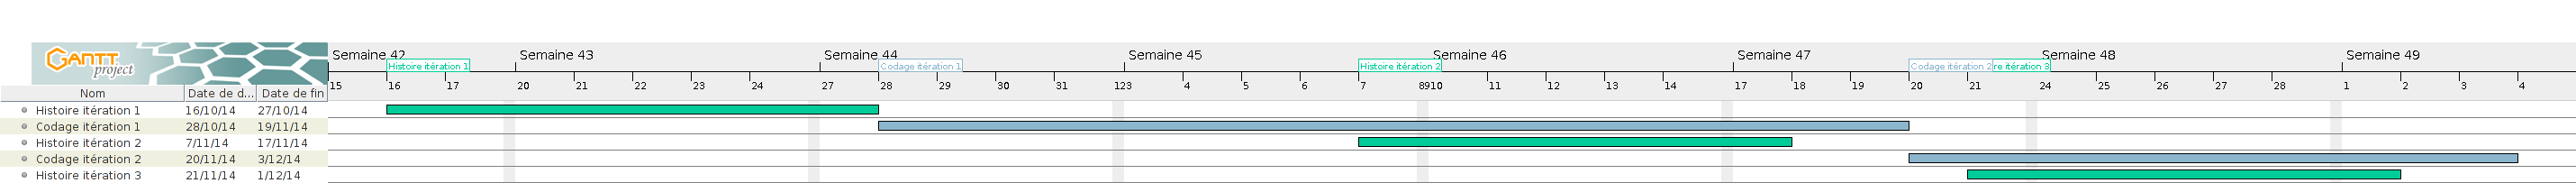
\includegraphics[scale=0.13]{images/gantt_projet_1er_quadri.png}
		\end{center}
		
		\begin{center}
			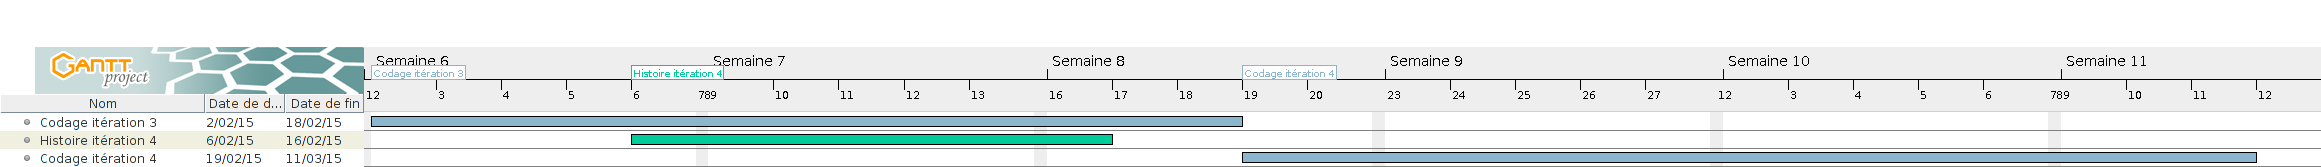
\includegraphics[scale=0.16]{images/gantt_projet_2eme_quadri.png}
		\end{center}
		
		
	\chapter{Première itération}
   		\section{Diagramme UML}
   			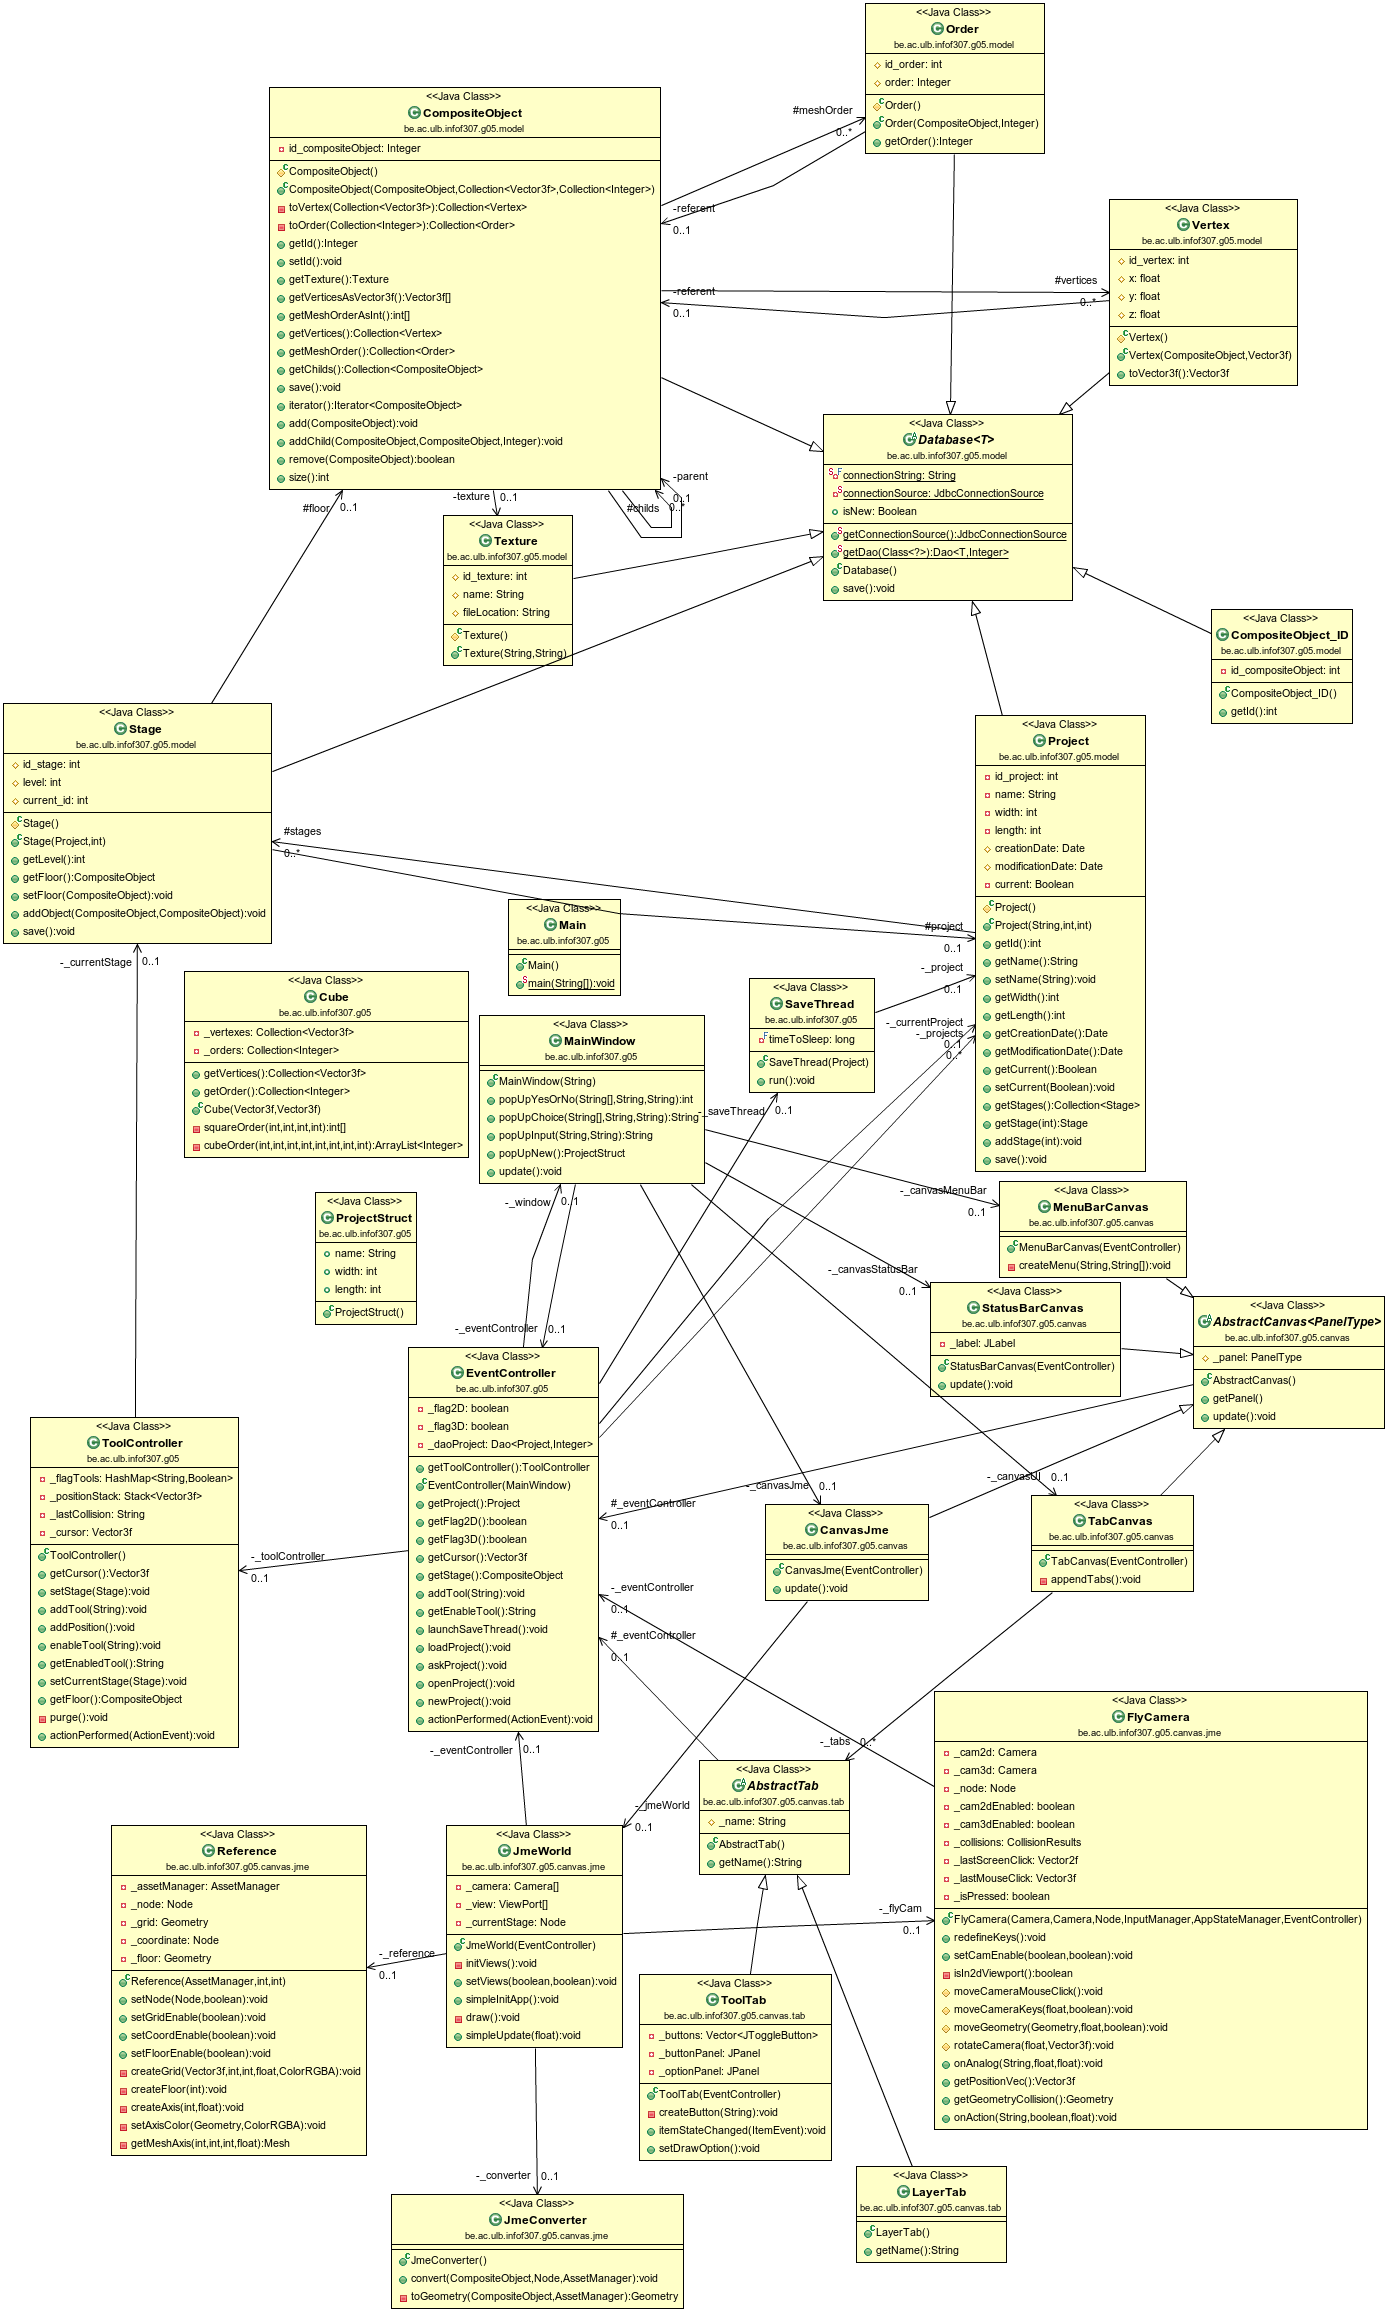
\includegraphics[scale=0.2]{images/uml.png}
		\section{Suivi de planification du projet}
			\subsection{Fonctionnalités}
				Toutes les fonctionnalités indiquées dans l'histoire de la première itération ont été implémentées. Ces fonctionnalités étaient de permettre à l'utilisateur : 
				\begin{itemize}
					\item De configurer la maison
					\item D'afficher la maison en 2D et 3D
					\item De se déplacer dans le projet en cours
					\item D'ouvrir/afficher et de modifier un ancien projet ou d'en créer un nouveau
					\item De faire des sauvegardes automatiques
				\end{itemize}
				
				Afin de réellement avoir un rendu de la maison en 2D et en 3D, les murs ont été implémentés. L'utilisateur peut donc commencer à créer les contours de sa maison, ainsi que les pièces.
			
			\subsection{Choix effectués}
				\paragraph{JMonkey} JMonkey a été choisi car il est très complet, open source, qu'il gère parfaitement l'affichage 3D et permet d'importer facilement tous les objets de l'histoire 5.
				\paragraph{Swing}
					Swing est la librairie graphique par défaut de Java, son utilisation s'est donc imposée pour la réalisation de la fenêtre de l'application d'architecture 3D.					
				\paragraph{Les Design Patterns} Afin de réaliser du code de qualité, les design patterns ont été employés. La réalisation générale de cette première itération repose ainsi entièrement sur le design MVC (modèle - vue - controleur). 
				\paragraph{La sauvegarde} Nous avons décidé d'utiliser une base de données afin de faciliter la sauvegarde des données. Elle nous permettra de faire l'abstraction de la sauvegarde et du chargement des données pour nous concentrer sur l'implémentation des fonctionnalités.
				
Notre application utilisera de manière intensive des objets en 3 dimensions et des textures. Nous avons décidé de ne pas les placer dans la base de données pour ne pas la saturer (à cause de la taille de ces fichiers) et pour offrir plus de flexibilité à l'utilisateur quant aux objets et textures qu'il pourra utiliser. Etant donné que nous avons choisi le modèle MVC (Model View Controller) pour structurer notre projet, cela permettra également de bien séparer le modèle de la vue en chargeant les objets en 3 dimensions et les textures dans la vue et en gérant leur emplacement dans le modèle.

Dans le cadre d'un projet stand-alone, nous avons décider d'utiliser la base de données SQLite \footnote{\url{http://www.sqlite.org}} car elle est open source, légère, rapide et se présente sous la forme d'un simple fichier, ce qui évite d'avoir à installer un serveur de base de données et donc permet de réduire les dépendances de notre application.

Pour plus de facilité dans l'utilisation de la base de données, nous utiliserons une bibliothèque ORM (Object Relational Mapping). Cela nous permettra de minimiser l'utilisation du SQL (Structured Query Language) et de faire abstraction de la base de données sous-jacente.

Nous avons choisi ORMlite \footnote{\url{http://ormlite.com/}} pour sa simplicité et son efficacité. ORMlite offre un bon support de plusieurs base de données open-source, ce qui nous autorise à changer de base de données en cas de besoin.

SQLite et ORMlite sont supporté par Java avec l'ajout de 3 fichiers JARs : un pour ORMlite, un pour l'interface entre ORMlite et JDBC (Java DataBase Connection, l'interface de connexion à une base de données de Java) et un pour le driver SQLite pour JDBC. Tout ceci ne nécessite aucune installation supplémentaire de la part de l'utilisateur.

			\subsection{Difficultés rencontrées}
				\paragraph{L'affichage :} Lors des premiers tests d'affichage en 2D et en 3D, le choix avait été fait de séparer l'écran de l'application en deux parties distinctes : le rendu 2D en haut et le 3D en bas. Cependant, la hauteur de chacune des images était alors divisée par deux, et ces dernières apparaissaient écrasées. De plus, comme la création de la maison se fait sur base du plan 2D, il semblait utile de pouvoir n'afficher que l'une des deux vues. C'est pourquoi, nous avons finalement décidé de permettre à l'utilisateur de n'afficher qu'une seule des deux vues au choix, mais aussi les deux en même temps avec la vue 3D apparaissant dans le coin inférieur droit de l'écran s'il le désirait.
				
				\paragraph{Les événements :} Les événements sont partagés entre Swing et JMonkeyEngine. Or il est parfois nécessaire de récupérer un premier clic sur un outil dans swing, suivi d'une suite de points à l'écran dans le canvas JME. Le passage des événements entre les deux librairies n'a pas été évident, ce qui conduira sans doute un à refactoring de la modèle et du contrôleur lors d'une itération future.
				
				%\paragraph{Le modèle :} TODO
				% En particulier, la partie "modèle" contient tous les éléments de la maison : les étages, le sol, les murs, les fenêtres, etc... Chacun de ces éléments étant une sous-partie d'un autre élément (le sol et les murs appartiennent à un étage, les fenêtres et les portes aux murs,...) un pattern Composite associé à un pattern Itérateur a été utilisé.

				%!--!
				%sauvegarde automatique : thread en plus ou sur le thread de l'affichage ? attention au lag si dans affichage.
				
				\paragraph{} La difficulté principale de cette première partie aura été de réussir à coder en tenant compte des prochaines itérations, afin de ne pas avoir à modifier le code pour y ajouter les objets et autres.
				
			\subsection{Dernière ligne droite}
				Quelques jours avant la remise, il reste à finaliser la première histoire. Afin de voir clairement les tâches à effectuer, voici un diagramme de Gantt les reprenant.
				\begin{center}
					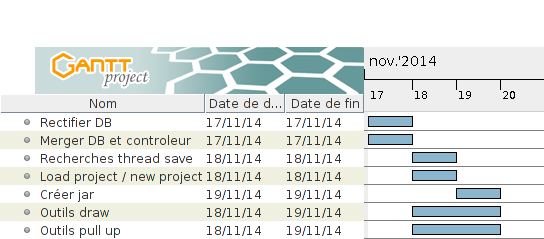
\includegraphics[scale=0.5]{images/gantt_it1.png}
				\end{center}	
				
		\section{Observations relatives à la première itération}
				Après cette première partie du projet, il apparaît que l'organisation d'un projet d'une telle ampleur doit être réfléchie et clairement mise en place. Les échéances de 2 semaines entre chaque remise obligent d'avoir un échange constant entre les différents membres du groupe : une seule réunion par semaine afin de voir l'avancement de chacun ne suffit pas. C'est pourquoi des groupe de conversation Skype on finalement été créés afin de permettre un meilleur échange. Le diagramme UML s'avère être la partie la plus importante : elle permet d'être sûr de la forme générale du code, avant de commencer à l'écrire. Sans lui, du code inutile risque d'être écrit puis supprimé, ce qui amène à une perte de temps inacceptable dans un projet à échéances si courtes. De plus, les tâches de chaque membres doivent être très clairement définies, sous peine de voir plusieurs membres coder la même chose ou de faire des choses inutiles. 
				
				Pour la seconde itération, une attention particulière sera donc donnée à l'organisation dès les premiers jours, afin de gérer au mieux le temps imparti, et de finir le travail bien à temps.
\end{document}
